\documentclass[10pt,a4paper]{article}
\usepackage[left=28.32bp,right=28.32bp,top=26.76bp,bottom=19.00bp]{geometry}
\usepackage{fontspec}
\setmainfont[FakeStretch=0.988]{Times New Roman}
\usepackage{graphicx}
\usepackage{eso-pic}
\usepackage{enumitem}
\usepackage[normalem]{ulem}
\renewcommand{\ULdepth}{3.30bp}
\usepackage{xcolor}
\usepackage{hyperref}
\hypersetup{colorlinks=true,urlcolor=blue,linkcolor=black,pdfborder={0 0 0}}

\pagestyle{empty}
\setlength{\parindent}{0pt}
\setlength{\parskip}{0pt}
\setlength{\emergencystretch}{1em}
\hyphenpenalty=10000
\exhyphenpenalty=50
\raggedbottom
\AtBeginDocument{\fontsize{9.12bp}{10.32bp}\selectfont}

\newcommand{\sectionrule}[1]{%
  \par\vspace{3.36bp}\noindent\textbf{#1}\par\vspace{2.62bp}%
  \hrule height 0.72bp\vspace{2.34bp}%
}
\newcommand{\compactsectionrule}[1]{%
  \par\vspace{0.24bp}\noindent\textbf{#1}\par\vspace{2.62bp}%
  \hrule height 0.72bp\vspace{0.66bp}%
}
\newcommand{\educompany}[2]{\par\noindent\textbf{#1}\hfill\textbf{#2}\par\vspace{1.44bp}}
\newcommand{\jobcompany}[2]{\par\vspace{1.92bp}\noindent\textbf{#1}\hfill\textbf{#2}\par\vspace{1.44bp}}
\newcommand{\titleline}[1]{\par\noindent\textbf{#1}\par}
\newcommand{\roleline}[2]{\par\noindent\uline{\textit{#1}}\hfill\textbf{#2}\par}
\newcommand{\eduroleline}[2]{\par\noindent\uline{\textit{#1}}\hfill\textbf{#2}\par\vspace{1.44bp}}
\newcommand{\venueline}[2]{\par\noindent\uline{\textit{#1}}\hfill\textbf{#2}\par}
\newenvironment{cvitems}{%
  \begin{itemize}[leftmargin=14.20bp,labelwidth=4.20bp,labelsep=10.00bp,align=left,
    topsep=0bp,itemsep=0bp,parsep=0bp,partopsep=0bp,label={\textbullet}]
}{\end{itemize}}
\newenvironment{subitems}{%
  \begin{itemize}[leftmargin=6.80bp,labelwidth=7.24bp,labelsep=13.76bp,align=left,
    topsep=0bp,itemsep=0bp,parsep=0bp,partopsep=0bp,label={\fontspec{Arial Unicode MS}➢}]
}{\end{itemize}}

\begin{document}
\fontsize{9.12bp}{10.32bp}\selectfont
\spaceskip=2.20bp plus 1.00bp minus 0.61bp
\xspaceskip=\spaceskip
\AddToShipoutPictureFG*{%
  \AtPageLowerLeft{\put(526.35bp,759.42bp){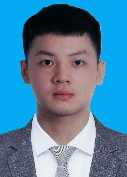
\includegraphics[width=41.478bp,height=58bp]{photo.png}}}%
}

\vspace*{-5.18bp}{\fontsize{16.08bp}{19.86bp}\selectfont\textbf{Zixi Jiang}}\par\vspace{4.08bp}
Email: \href{mailto:jiangzixi1527435659@gmail.com}{jiangzixi1527435659@gmail.com} \enspace|\enspace Tel: +86 19116411259\par
\href{https://www.linkedin.com/in/zixijiang/}{LinkedIn} \enspace|\enspace
\href{https://scholar.google.com/citations?user=31Lf3w8AAAAJ\&hl=zh-CN\&oi=sra}{Google Scholar} \enspace|\enspace
\href{https://yichuanalex.github.io/}{Personal Website}\par

\sectionrule{EDUCATION BACKGROUND}
\educompany{Clemson University}{SC, USA}
\eduroleline{Ph.D of Computer Engineering \& Research Assistant}{09/2026 -- 06/2031}
\begin{cvitems}
\item \textit{Ph.D. student supervised by Prof. Lan Zhang, focusing on wireless AI systems, distributed learning, secure federated learning, and intelligent edge networks.}
\end{cvitems}

\educompany{University of Jyväskylä}{JYV, FIN}
\eduroleline{Summer School}{07/2026 -- 08/2026}
\begin{cvitems}
\item \textbf{Major Courses:} \textit{Entrepreneurship Opportunities in Blockchain Technology}
\end{cvitems}

\educompany{East China Normal University}{SH, CN}
\eduroleline{Research Assistant}{05/2025 -- 05/2026}
\begin{cvitems}
\item \textit{Supervised by Prof. Chunyang Wang \& Prof. Xiang Li, conducted research on Generative Recommender Systems, Graph Neural Networks (GNNs), and Multi-Agent Systems, focusing on enhancing recommendation accuracy and optimizing collaborative decision-making mechanisms.}
\end{cvitems}

\educompany{Shanghai Jiao Tong University}{SH, CN}
\eduroleline{Research Assistant}{05/2024 -- 10/2024}
\begin{cvitems}
\item \textit{Supervised by Prof. Dongdong Ge, researched mathematical optimization algorithms for the Cardinal Optimizer (COPT), analyzing numerical stability and improving solution efficiency for linear programming problems.}
\end{cvitems}

\educompany{Anhui University}{AH, CN}
\eduroleline{B.Sc of Science in Data Science \& Big Data Technology}{09/2022 -- 06/2026}
\begin{cvitems}
\item \textbf{Major Courses:} \textit{College Physics, Advanced Mathematics, Linear Algebra, Circuits and Electronics Technology, Discrete Mathematics, Probability Theory and Mathematical Statistics, Fundamentals of Big Data Analytics Language, Data Structure, Design and Analysis of Algorithms, and Linux operating systems and Applications}
\item \textbf{GPA: 3.53}
\item \textbf{RANK: 5\%}
\end{cvitems}

\sectionrule{SKILLS}
\begin{cvitems}
\item Coding skills:
  \begin{subitems}
  \item Proficient in front and back end full stack development, such as: C++, Python, JavaScript, HTML, SQL, Java, CSS, C\#, R and VUE
  \item Up to two years of data warehouse skills, proficient in Microsoft big data development and analysis tools, such as: Hadoop, Spark, Databricks
  \item Master multiple project experience of deep learning algorithm deployment and full-cycle large model training under multi-operating systems and domestic and foreign hardware environments
  \item Good at mathematical modeling and the use of solvers at home and abroad, such as: MATLAB, CPLEX, Gurobi, COPT
  \end{subitems}
\item Language skills:
  \begin{subitems}
  \item TOEFL:106/120, Reading:30/30, Listening:29/30, Speaking:23/30, Writing:24/30
  \end{subitems}
\item Management ability:
  \begin{subitems}
  \item Management experience in three IT projects for L 'Oreal and KPMG
  \end{subitems}
\item Enterprise financing ability:
  \begin{subitems}
  \item 3 years of self-financing ability and excellent communication skills
  \item Good at social engineering
  \end{subitems}
\end{cvitems}

\vspace{-1.35bp}\sectionrule{INTERNSHIP EXPERIENCE}
\jobcompany{DiDi Global Inc.}{Strategic \& Business Analysis Department}
\roleline{Commercialization Strategy \& Operations Officer}{06/2026 -- Present}
\begin{cvitems}
\item Spearheaded AI-centric strategic research by tracking product-market dynamics and evaluating innovative AI applications; synthesized findings into comprehensive reports to deliver actionable insights to core management and business teams.
\item Conducted in-depth competitive intelligence analysis through secondary research and expert interviews; systematically collected and interpreted competitor data to identify market trends and strategic opportunities.
\item Scouted and engaged with AI startups across global markets; analyzed strategic layouts of major tech players to identify high-potential investment and partnership targets.
\end{cvitems}

\jobcompany{Shanghai Xuanling Asset Management Co., Ltd.}{Investment Department}
\roleline{CTA Strategy Investment Manager}{02/2026 -- 06/2026}
\begin{cvitems}
\item Responsible for the shenzhen stock exchange Level - 2 weaves dish data retrieval, the complete dynamic visualization harden seal deals, queue, microstructure analysis support for the policy; Tracking emersion head broker research and strategy, refining the core assumptions and to carry out quantitative inspection; Based on factor investment framework, build and back-test idiosyncratic volatility (IVol) factors such as style, participation factor combination optimization and IC/IR analysis; Use Python (Pandas, NumPy, scikit - learn) to complete the data cleaning, factor calculation, to help build more factor stock selection model; Familiar with quantitative research process, data preprocessing, factor development, back to the test certificate, strategy evaluation and online data quality control experience.
\item Track the development of CTA (including over ten sub-strategies with low correlation), build a stock multi-factor framework and complete the backtesting of the stock selection strategy; The strategy covers all types of futures, mainly focusing on the 10-14 day medium-long term cycle, forming over thirty sub-strategy pools, and holding 60+ varieties daily. Responsible for the real-time execution and tracking of CTA, manage the CTA No.2 product (established at the end of 2022, with an annualized return \textgreater{} 27\%, and the maximum drawdown is approximately 12\%); Complete the connection of the trading system, realize the automatic deployment of the strategy, and dynamically adjust the position ratio (regular \textless{} 5\%, special \textless{} 10\%). Relying on the multi-hedging, leverage and crisis alpha attributes of CTA, multi-cycle and multi-variety allocation reduces correlation, strictly control the drawdown, and ensure the stability of the strategy.
\end{cvitems}

\jobcompany{Volkswagen Group}{ADAS,CARIAD China}
\roleline{ADAS System Engineer}{09/2025 -- 02/2026}
\begin{cvitems}
\item Deeply participate in the ADAS data closed-loop project, and for the next-generation L2+/L3 ADAS functions, conduct batch processing on test vehicles to build an integrated data closed-loop of vehicle-cloud-scene. Connect the entire chain (refer to true value sensor modification → bypass data acquisition at the vehicle end → cloud data lake → scene reconstruction → KPI visualization) to provide a replicable data toolchain for SOP models in 2026
\item Based on the truth data of CARIAD Small Loop, a three-stage world model training pipeline of ``offline - closed loop - distillation'' was built. Data augmentation was carried out by calling the GAIA-1 derivative script based on the OrienLink platform. Expand 0.2TB of real vehicle data to an\newpage
8TB virtual long-tail scene (such as heavy rain, construction, spillage from the preceding vehicle, etc.), and automatically generate the future 5-\linebreak
second occupation raster and optical flow with 4D-BEV annotations; The OpenScenario/OpenDrive scenario was injected into the CARLA-\linebreak
Cosmos co-simulator, and the end-to-end driving strategy was trained with reinforcement learning (Dreamer-V3) for closed-loop simulation. The\linebreak
success rate of 1000 corner-cases decreased from 41\% to 87\%. The 1.1B parameter world model was distilled at the vehicle end into a lightweight\linebreak
Safety-WorldNet with 35 M parameters and deployed to the TDA4VH MCU. With a loop delay of 38 ms, real-time fail-safe verification was\linebreak
performed on the J6 domain control, reducing the false braking rate by 19\%
\end{cvitems}

\jobcompany{Bosch (China) Investment Co., LTD}{ETAS(Shanghai) Co., LTD}
\roleline{Intelligent Driving Engineer}{03/2025 -- 08/2025}
\begin{cvitems}
\item Integrate the requirements of multiple automotive manufacturers (XPeng, Lotus, NIO, Tesla), develop an Embedded AI Coder, and tune the neural network to adapt to the C code of various microcontrollers and microprocessors. Outstanding speed and efficient memory usage ensure that high-quality artificial intelligence models can be deployed within embedded systems
\item Develop a modular and scalable driving assistance module platform to collect data, measure large datasets, and reduce the demand for ECU computing resources. Support early and continuous development through integrated hardware and software tools, and provide highly customized solutions through defined APIs
\end{cvitems}

\jobcompany{L 'Oreal (China) LTD}{Department of Beauty Science and Technology}
\roleline{Operational Project Management}{08/2024 -- 02/2025}
\begin{cvitems}
\item Responsible for coordinating data suppliers such as Publicis and Giant Engine to carry out multidimensional data cleaning, build high-quality data sets, and carry out accurate portrait training for three sets of large models for different L 'Oreal user groups, establish personalized customer relationships through data-driven user insights, and effectively improve TikTok customer loyalty and secondary repurchase rate
\item Fully monitor project upstream and downstream data flows to ensure data security and compliance
\item Coordinate multi-party data suppliers and internal teams, integrate resources to promote project implementation, efficiently complete key links such as data cleaning and model training, and ensure project delivery on time
\end{cvitems}

\jobcompany{KPMG Huazhen LLP (Special General Partnership)}{IT Advisory Department}
\roleline{Cloud Computing Architecture Design Project Manager}{11/2023 -- 07/2024}
\begin{cvitems}
\item As a team member, I designed the Microsoft cloud computing service middleware architecture suitable for different automotive manufacturers (such as JAC and FAW-Volkswagen), and proposed multiple edge middleware solutions as well as high-performance and scalable data collection and processing solutions
\item Conduct a large number of test cases to verify the reliability of cloud services after migration and deliver a large number of technical manuals
\item The whole process supervises the project team to deliver the project orderly at all time nodes to ensure the project is completed on time and with high quality
\end{cvitems}

\sectionrule{ENTREPRENEURSHIP EXPERIENCE}
\jobcompany{Huake Yunlian (Beijing) Technology Co., Ltd}{}
\roleline{CTO}{05/2023 -- 02/2025}
\begin{cvitems}
\item Use the technical achievements of the start-up team to invest in technology, help the company establish the early business solutions, and lay the technical foundation and business direction for the company's development
\item Obtained commercial orders from Xinjiang and Shanghai State Grid through multiple sales orders, and obtained technical and economic investment by relying on college student venture fund and innovation and entrepreneurship competition, so as to promote the company's business expansion and capital accumulation
\item Transform technological achievements into patents, soft books and papers, realize the realization of results, and realize the company's value enhancement and long-term development by optimizing the ownership structure
\end{cvitems}

\compactsectionrule{SCIENTIFIC RESEARCH EXPERIENCE}
\titleline{PIVOT: Risk-Controlled Routing of Verifier Feedback for Reliable Policy Improvement}
\venueline{ICLR 2027 Conference Submission, Under Review}{05/2026 -- present}
\begin{cvitems}
\item Developed PIVOT, an optimizer-aware verifier routing framework for reliable LLM post-training that selects heterogeneous feedback sources based on both verifier reliability and the expected direction of the induced policy update. Integrated executable tests, reward models, generative judges, and retrieval critics through a unified preference-graph interface with sequential acquisition, escalation, and abstention. Across two LLMs and four reasoning domains, PIVOT achieved 68.4 trusted utility, improving over BayesianRouter-H and uncertainty routing by 1.6 and 2.3 points, respectively, while maintaining 0.047 GG-risk at 82\% coverage.
\item Designed a LoRA-space update-alignment mechanism using optimizer-native virtual gradients and JL projection, combined with calibrated verifier correctness and reliability-adjusted feedback weighting. Introduced a finite-sample risk certificate with minimum coverage constraints and phase-wise recertification to control erroneous feedback admission under policy drift. Comprehensive ablation, optimizer-transfer, and cost analyses validated the contributions of directional alignment, reliability calibration, certification, and adaptive escalation.
\end{cvitems}

\titleline{DeepLNP: role-aware dual-path learning for lipid nanoparticle delivery efficacy modelling and within-screen ranking}
\venueline{Briefings in Bioinformatics, Under Review}{03/2026 -- present}
\begin{cvitems}
\item Developed DeepLNP, a discriminative deep learning system for accurate prediction of LNP key properties (transfection efficiency, particle size, zeta potential, cytotoxicity) to address the inefficiencies of traditional trial-and-error formulation development. Integrates multi-modal data via an innovative four-component encoding architecture, cross-attention and MoE-based fusion, and multi-task learning. Achieves state-of-the-art performance on a curated dataset, outperforming existing baselines and accelerating mRNA and gene therapy development.
\item Engineered a four-component MPNN encoder with molar ratio-weighted fusion to capture component synergies and enhance interpretability. Implemented a hierarchical multi-modal fusion module with cross-attention and adaptive expert weighting. Adopted uncertainty-weighted multi-task learning for improved generalization. Designed a feature priority mechanism to ensure stable performance under different data availability conditions.
\end{cvitems}

\titleline{SourceGuard-Gait: Claim-Bounded Invariance for Heterogeneous Public-Source Abnormal-Gait Screening}
\venueline{AAAI 2027 Conference Submission, Under Review}{10/2024 -- present}
\begin{cvitems}
\item The work content of this paper is to propose a model called AdaptiveGaitSegNet, which is used to accurately identify the gait of patients with Parkinson's disease and address the limitations of traditional assessment methods. This model integrates techniques such as data preprocessing, dual-branch feature extraction, multi-scale feature fusion, and joint loss function to comprehensively analyze the gait of PD. Experiments on the GAIT-IT and GAIT-IST datasets show that the model performs exceptionally well in terms of accuracy, precision, recall rate, and F1 score, outperforming other advanced models and demonstrating high practical application value.
\item This paper designs a dual-branch feature extraction mechanism, extracting local frame features and global sequence features respectively, and fusing the features through residual connections. Introduce the focus convolution operation to accurately capture the local motion features of different parts of the human body, avoiding the feature blurring problem of traditional convolution. The edge-aware pooling method is adopted to dynamically adjust the pooling operation and enhance the capture of edge information. By applying multi-scale pyramid pooling, the multi-scale features of gait are comprehensively captured to enhance the model's adaptability to complex scenarios. A joint loss function is proposed, combining triplet loss and cross-entropy loss to optimize the geometric structure of the feature space and enhance classification performance. These\newpage
innovations have significantly enhanced the robustness and recognition accuracy of the model.
\end{cvitems}

\vspace{1.92bp}\titleline{Graph Attention Network-Based Multi-Omics Data Integration for Precise Key Gene Prediction in Triple-Negative Breast Cancer}
\venueline{IEEE/ACM Transactions on Computational Biology and Bioinformatics (SCI), Apr 2026}{07/2024 -- 05/2025}
\begin{cvitems}
\item This paper addresses triple-negative breast cancer (TNBC) with a multi-omics framework using Graph Attention Network (GAT) to predict key genes and improve prognosis. It integrates single-cell RNA-seq, chromatin accessibility, and radiomics data. After quality control and standardization, features are extracted via PCA and UMAP dimensionality reduction. Cell types are annotated using CellMarker 2.0. Canonical correlation analysis aligns multi-omics features to build a multimodal gene network including gene homology, PPIs, and transcription factor networks. Multi-head attention captures gene interactions, highlighting key modules, and CellphoneDB analyzes intercellular communication. The model is validated on external datasets, with hyperparameters optimized for robustness and generalization. Pathway enrichment links key genes to TNBC biological processes. An MLP model stratifies patient risks and verifies clinical relevance.
\item The GAT-MLP prognostic model was developed by integrating single-cell RNA sequencing (scRNA-seq), assay for transposase-accessible chromatin sequencing (ATAC-seq), and radiomics data. This integration extends the application of graph attention networks (GAT) in oncology research and enhances the precision of key gene identification through multi-head attention mechanisms. The model synergistically combines intercellular communication analysis with transcription factor regulatory networks to elucidate tumor microenvironment mechanisms. A\\
multimodal feature matrix, constructed via canonical correlation analysis (CCA) alignment, enhances the capture of complex gene relationships. This framework enables stratification of triple-negative breast cancer (TNBC) patients into distinct risk groups, thereby providing clinically validated biomarkers and therapeutic targets. Systematic hyperparameter optimization, implemented through grid search and cross-validation, ensures model stability and generalization capability. Variational Dropout enhances robustness, mitigates overfitting, and improves handling of high-dimensional data.
\end{cvitems}

\vspace{1.92bp}\titleline{A Named Entity Recognition Method for Tea Plant Pests and Diseases Based on BERT-BiLSTM-CRF}
\venueline{Transactions of the Chinese Society for Agricultural Machinery (EI), July 2025}{05/2023 -- 05/2024}
\venueline{National Invention Patent (2025104224368), In Substantive Examination}{07/2024 -- 05/2025}
\venueline{Copyright of Computer Software (2024SR0720539), Aug 2024}{07/2024 -- 05/2025}
\begin{cvitems}
\item This study built a high-quality dataset for Chinese tea tree pests and diseases using multi-source heterogeneous data, laying the foundation for subsequent research. A BERT-BILSTM-CRF-based named entity recognition method was proposed, combining BERT's pre-training, BiLSTM's sequence modeling, and CRF's global optimization to significantly improve accuracy and efficiency, performing well on self-built and general datasets. A knowledge graph was constructed, with knowledge stored in Neo4j for visualization and effective management. Finally, an intelligent question-answering system was developed, providing users with efficient knowledge acquisition and decision support.
\item An innovative BBC model-based method is proposed for identifying named entities of tea tree pests and diseases, combining BERT's pre-training, BiLSTM's sequence modeling, and CRF's global optimization. This significantly improves recognition accuracy and efficiency. A knowledge graph of tea tree pests and diseases has been constructed, integrating multi-source heterogeneous data for structured organization and supporting applications like intelligent question answering. An intelligent question answering system, based on this knowledge map, integrates the BBC and BertForSequenceClassification models to handle question understanding, knowledge retrieval, and answer generation, providing an efficient tool for decision-making on pest and disease control.
\end{cvitems}

\vspace{2.16bp}\compactsectionrule{PROJECT EXPERIENCE}
\titleline{Vehicle Trajectory Prediction System Based on Graph-WaveNet}
\venueline{Copyright of Computer Software (2025SR0673325), Aug 2024}{12/2022 -- 05/2023}
\begin{cvitems}
\item Based on algorithmic optimization, this project effectively processes and utilizes vehicle trajectory and external environmental factor data to enhance prediction accuracy and model interpretability. By introducing the adaptive graph convolutional network (GraphWaveNet), the model can dynamically construct the adjacency matrix of physical associations among vehicle entities, thereby autonomously learning the potential dependencies among factors. This method does not require manual predefined association rules, significantly enhancing the flexibility and accuracy of factor relationship mining. The predictors generated in the first stage are taken as covariates of the time series, and then feature fusion is carried out with the trajectory data to construct a dataset that simultaneously contains structured information and dynamic trajectory features. This dataset is input into the Time Series Dense Encoder (TiDE) model, and the final output trajectory prediction results.
\end{cvitems}

\titleline{A Fault Wave Analysis Method for Industrial Substation Closing Resistors Based on Convolutional Neural Network}
\venueline{National Invention Patent (202410432228.1), Sept 2025}{07/2024 -- 05/2025}
\venueline{Copyright of Computer Software (2024SR0719404), Aug 2024}{04/2023 -- 08/2023}
\venueline{Copyright of Computer Software (2024SR0726917), Aug 2024}{04/2023 -- 08/2023}
\begin{cvitems}
\item This study proposes an innovative application of Convolutional Neural Networks (CNNs) for identifying fault types in distribution network closing resistor recordings. A novel methodology combines the Hilbert-Huang Transform (HHT) for fault signal processing, utilizing the resulting real-time spectrogram as the CNN input. This approach significantly enhances the processing capability for non-stationary signals while circumventing the limitations associated with wavelet basis function selection. A seven-layer CNN architecture was designed and trained using the Adam optimization algorithm. Adaptive learning rate adjustment and regularization techniques were introduced to accelerate model convergence while improving recognition accuracy and stability. Validation through PSCAD/EMTDC simulations under diverse practical operating conditions demonstrates that this method achieves significant improvements in fault identification accuracy, enhances generalization capability and robustness, and exhibits strong adaptability to complex operating scenarios.
\end{cvitems}

\compactsectionrule{AWARDS}
\begin{cvitems}
\item Received the First Prize (Team) in the UBIQUANT CHALLENGE AI Reasoning Competition in 2026
\item Project Leader of the National College Students' Innovation and Entrepreneurship Project in 2024
\item Received the Excellence prize in the China Industrial Internet Research Institute's first ``Tongzhi Cup'' Artificial Intelligence Innovation and Application Competition in 2023
\item Received the First prize in the 18th ``Challenge Cup'' National College Students' Extracurricular Academic Science and Technology Works Competition in 2023
\item Received the Second prize in the 14th Blue Bridge Cup Team Competition in 2023
\item Received the Second Prize of the National College Student Information Security Anhui Provincial Competition under the Provincial level in 2023
\item Received the Provincial Silver award in the 17th ICAN National College Student Innovation and Entrepreneurship Competition in 2023
\item Anhui University 2023 Outstanding Student Scholarship
\item Received the 9th Anhui Province ``Internet +'' College Student Innovation and Entrepreneurship Competition Finals Provincial Gold Award in the main track of colleges and universities in 2022
\end{cvitems}

\end{document}
